\documentclass{article}

%%% Defines %%%%%%%%%%%%%%%%%%%%%%%%%%%%%%%%%%%%%%%%%%%%%%%%%%%%%%%%%%%%%%%%%%%%

\usepackage{graphicx}
\usepackage{tikz}
\usepackage{pgfplots}
\pgfplotsset{compat=1.18}
\usetikzlibrary{shapes.misc}
\usepackage[european,straightvoltages]{circuitikz}
\usepackage[T1]{fontenc}
\usepackage[ngerman]{babel} 
\usepackage[colorlinks]{hyperref}
\usepackage{caption, float, subcaption}
\usepackage{xcolor}
\usepackage{setspace}
\usepackage{mathtools, amssymb, ntheorem, amsmath, siunitx}
\sisetup{per-mode=fraction, separate-uncertainty=true,exponent-base=10,output-decimal-marker={,}}
\DeclareSIUnit\liter{l}
\usepackage{enumitem}
\usepackage{minted}
\usepackage{placeins}

\usepackage{tikz-uml}

% manuelle hyponation
\hyphenation{Än-de-run-gen}


% maths
\newcommand{\abs}[1]{\left| #1 \right|}
\newcommand{\br}[1]{\left( #1 \right)}
\newcommand{\ubar}[1]{\mkern 1.5mu\underline{\mkern-1.5mu#1\mkern-1.5mu}\mkern 1.5mu}

% image
\newcommand{\img}[5]{
    \begin{figure} [#5]
    \centering
    \includegraphics[width=#2\linewidth]{#1}
    \caption{#3}
    \label{pic:#4}
    \end{figure}
}

% tikz
\newenvironment{gfx}[3]
{
    \newcommand{\gfxname}{#2}
    \newcommand{\gfxcaption}{#1}
    \begin{figure} [#3]
    \centering
    \begin{tikzpicture}
}
{
    \end{tikzpicture}
    \caption{\gfxcaption}
    \label{gfx:\gfxname}
    \end{figure}
}

\newcommand{\opt}{\ensuremath{\parallel}}

% cicuitikz
\newenvironment{ckt}[3]
{
    \newcommand{\cktname}{#2}
    \newcommand{\cktcaption}{#1}
    \begin{figure} [#3]
    \centering
    \begin{circuitikz}
	\draw
}
{
	;
    \end{circuitikz}
    \caption{\cktcaption}
    \label{ckt:\cktname}
    \end{figure}
}

% Code
\newfloat{Code}{htbp}{loc}
\floatname{Code}{Quelltext}
\definecolor{LightGray}{gray}{0.9}
\newenvironment{code}[4]
{%
  \VerbatimEnvironment
  \begin{Code} [#4]
  \caption{#2}%
  \label{cod:#3}%
  \begin{minted}[frame=lines,framesep=2mm,baselinestretch=1.2,bgcolor=LightGray,fontsize=\footnotesize,style=emacs]{#1}%
}
{%
  \end{minted}%
  \vspace{-20pt}%
  \end{Code}%
}
\makeatletter
\AtBeginEnvironment{minted}{\dontdofcolorbox}
\def\dontdofcolorbox{\renewcommand\fcolorbox[4][]{##4}}
\makeatother
\newcommand{\listofcode}{
  \doublespacing
  \listof{Code}{Quelltextverzeichnis}
}

%%% Head %%%%%%%%%%%%%%%%%%%%%%%%%%%%%%%%%%%%%%%%%%%%%%%%%%%%%%%%%%%%%%%%%%%%%%%

\title{Title}
\author{Benjamin Brohs, Kevin Hecke, Justin Meng}
\date{Date}

\setlength{\parindent}{0pt}
\setlength{\parskip}{1em}

\begin{document}

%%% Title %%%%%%%%%%%%%%%%%%%%%%%%%%%%%%%%%%%%%%%%%%%%%%%%%%%%%%%%%%%%%%%%%%%%%%

\begin{titlepage}
  \centering
	\begin{tabular}{lcr}
		
\includegraphics[width=0.35\textwidth]{fachbereich.png} & \hspace{0.195\textwidth} & 
\includegraphics[width=0.35\textwidth]{Q04_HTW_Berlin_Logo_quer_pos_FARBIG_RGB.jpg}\\
	\end{tabular}	
	\\[3cm]
	\Large
	Belegarbeit\\
	\vspace{2cm}
	\textbf{Minecraft-One-Week-Challenge Reloaded}\\
	\vspace{2cm}
	\begin{tabular}{ll} 
		Im Studiengang: & Computer Engineering \\		
	\end{tabular}	
	\\[3cm]
	\normalsize
	\begin{tabular}{ll}
	      \textbf{Erstellt von:} & Benjamin Brohs, Kevin Hecke, Justin Meng \\
        \textbf{Modul:} & Softwaretechnik \\
        \textbf{Semester:} & Sommersemester 2025 \\
	\textbf{Dozent:} & Thomas Baar
	\end{tabular}	
\end{titlepage}

\tableofcontents

\newpage

%%% Inhalt %%%%%%%%%%%%%%%%%%%%%%%%%%%%%%%%%%%%%%%%%%%%%%%%%%%%%%%%%%%%%%%%%%%

\section{Meilenstein 1} \label{sec:ms1}

Meilenstein 1 befasst sich mit der Beschreibung der Software, wie sie ohne die Änderung aufgebaut ist. Sowohl textuell, als auch per Modell.

\subsection{Informelle Beschreibung} \label{subsec:inf}

Die ausgewählte Software ist ein Projekt eines YouTubers, in einer Woche einen Klon des bekannten Spiels \href{https://www.minecraft.net}{Minecraft} zu programmieren. Bei dem Spiel Minecraft handelt es sich um ein sogenanntes Open-World Survival Game. Das bedeutet, der Spieler findet sich in einer algorithmisch generierten Welt wieder, die frei von dem Spieler erkundet werden kann. In dieser Welt hat der Spieler die Aufgabe gegen KI-gesteuerte Monster zu überleben. Zudem ist Minecraft für den stilisierten Grafikstil bekannt, der durch die Verwendung von quadratischen Blöcken und pixeligen Texturen geprägt ist.

Eben diese Eigenschaften wurden aufgegriffen und in einer einfachen C++ Umgebung mithilfe von OpenGL nachgeahmt. Der Spieler wird auch hier in eine generierte offene Welt gesetzt und kann sich darin frei bewegen und erkunden. Dem Spieler ist es dabei möglich, in alle Richtungen zu laufen, über Hindernisse zu springen, und zu sprinten und zu schleichen. Die Welt in der sich der Spieler bewegt, generiert auch einige Gewässer verschiedener Grö\ss{}en, in dieser Instanz des Spiels ist es dem Spieler aber nicht möglich darin zu schwimmen. Nun kann der Spieler diese Welt auch nach belieben verändern. Weniger komplex als im Basis Spiel, kann der Spieler ohne Bedingungen jeden Block aufnehmen und woanders wieder platzieren. Da dieses simple Projekt noch keine Benutzeroberfläche, wie z.B. ein Pause-Menü bietet, werden weiter Funktionen implementiert, um die Eingaben der Maus im Spiel zu Blockieren.

Die Spielwelt selber wird mithilfe von Rauschfunktionen generiert, spezieller einer Art Value-Noise. Damit soll die Generierung des Geländes natürlicher wirken. Zudem gibt es verschiedene Biome in der Welt, die ebenso zufällig verstreut sind und mit sich verschiedene Strukturen von Vegetation und unterschiedliche Arten von Blöcken mitbringen. So gibt es zum Beispiel Wüsten, in denen Kakteen wachsen oder Wälder in denen Bäume stehen.

In dieser Kopie des Spiels sind einige Haupt Eigenschaften noch nicht umgesetzt. Es gibt keine weiteren Spiel-gesteuerten Entitäten wie die Monster und Tiere im Basis Spiel. Auch hat der Spieler nicht die Möglichkeit Schaden zu nehmen, zu schwimmen, in sein Inventar zu schauen oder verschiedene Materialien und Werkzeuge herzustellen. Das Projekt verfolgt nicht das Ziel, ein vollständiges Spiel zu sein, sondern entstand im Rahmen einer technischen Herausforderung. Es dient in erster Linie als Grundlage für Lernzwecke, zur Analyse grundlegender Spielmechaniken sowie als Ausgangspunkt für mögliche Erweiterungen durch Dritte. Das Original Open-Source-Projekt ist zu finden unter \url{https://github.com/Hopson97/MineCraft-One-Week-Challenge}.

\subsection{Use-Case-Modell} \label{subsec:usecase}

Folgender Abschnitt thematisiert das UseCase Modell der Software. Es handelt sich hier um ein Spiel, das alleine gespielt wird, somit gibt es hier auch nur einen Akteur. Abbildung \ref{gfx:usecase} zeigt die UseCases, die in der Software implementiert sind. Diese sind in den folgenden Abschnitten näher beschrieben.

\begin{gfx}{UseCase Diagramm}{usecase}{ht}
  % Systemgrenze
  \begin{umlsystem}[x=4, y=0]{Minecraft-Klon}
    \umlusecase[x=0, y=0]{Bewegen}
    \umlusecase[x=0, y=-1.5]{Springen}
    \umlusecase[x=0, y=-3]{Flugmodus umschalten}
    \umlusecase[x=0, y=-4.5]{Maussteuerung deaktivieren}
    \umlusecase[x=0, y=-6]{Block abbauen}
    \umlusecase[x=0, y=-7.5]{Block platzieren}
  \end{umlsystem}

  % Akteur
  \umlactor[x=-2, y=-4.5]{Spieler}

  % Assoziationen
  \umlassoc{Spieler}{usecase-1}
  \umlassoc{Spieler}{usecase-2}
  \umlassoc{Spieler}{usecase-3}
  \umlassoc{Spieler}{usecase-4}
  \umlassoc{Spieler}{usecase-5}
  \umlassoc{Spieler}{usecase-6}
\end{gfx}

\newpage

\subsubsection*{Physikalische Rahmenbedingungen der Spielfigur}

Die Bewegung der Spielfigur basiert auf einem kontinuierlichen Physikmodell, das zwischen horizontaler und vertikaler Bewegung sowie zwischen Flug- und Bodenmodus unterscheidet. Die Geschwindigkeit in jeder Raumrichtung wird in jedem Simulationsschritt auf Basis folgender Prinzipien berechnet:

\begin{itemize}
  \item \textbf{Horizontale Bewegung:}  Eingaben wie Bewegungstasten erzeugen eine gerichtete Beschleunigung basierend auf der Blickrichtung der Spielfigur. Diese wird auf die aktuelle Geschwindigkeit addiert. Unabhängig vom Zustand (am Boden, in der Luft, im Flugmodus) wird eine konstante Dämpfung angewandt, die die Geschwindigkeit über die Zeit exponentiell reduziert.

  \item \textbf{Vertikale Bewegung:}  Diese unterscheidet sich je nach Modus: im \textbf{Flugmodus} gilt die gleiche Dämpfung wie in horizontaler Richtung. Die Eingaben \texttt{Springen} (Leertaste) und \texttt{Schleichen} (Strg) erzeugen eine gerichtete Beschleunigung nach oben oder unten, analog zu Bewegungseingaben horizontal. Im \textbf{Bodenmodus} gilt diese Dämpfung nicht mehr, stattdessen wird eine Gravitationskonstante von der vertikalen Geschwindigkeit subtrahiert. Ein Sprung setzt dann die vertikale Geschwindigkeit ohne eine Beschleunigung auf einen festen positiven Wert.

  \item \textbf{Zusammenfassung der Logik:}
  \begin{itemize}
    \item Dämpfung wirkt \textbf{immer} in allen Richtungen au\ss{}er vertikal im Bodenmodus.
    \item Gravitation ersetzt im Bodenmodus die vertikale Dämpfung.
    \item Sprung ist eine \textit{diskrete Initialisierung der vertikalen Geschwindigkeit}, kein kontinuierlicher Prozess.
    \item Die Dämpfung erfolgt exponentiell, die Gravitation linear.
  \end{itemize}
\end{itemize}

\textit{Hinweis:} Diese Mechaniken gelten systemweit und werden innerhalb der Use Cases nicht vollständig modelliert, sondern vorausgesetzt. Ihre konkrete Auswirkung auf das Spielerlebnis ergibt sich aus dem Zusammenspiel dieser physikalischen Regeln mit den Eingaben des Spielers.

\newpage

\subsubsection*{UC01 – Bewegen}

\textbf{Name:} Bewegen \\
\textbf{Akteur:} Spieler \\
\textbf{Ziel:} Fortbewegung der Spielfigur in der Spielwelt entsprechend der Eingaben \\
\textbf{Vorbedingungen:} Spiel läuft, Spielfigur ist aktiv, Spielfigur schaut in eine ausgewählte Blickrichtung \\
\textbf{Nachbedingungen:} Position der Spielfigur wurde ggf. angepasst \\
\textbf{Beschreibung:} Der Spieler bewegt die Spielfigur durch Eingabe von Bewegungstasten. Die Bewegungsrichtung wird durch die aktuelle Blickrichtung bestimmt. Der Use Case bleibt aktiv, solange Eingaben erfolgen. Sprinten, Schleichen sowie vertikale Flugbewegung (Flugmodus aktiv) beeinflussen die Fortbewegung.

\textbf{Ablaufspezifikation:}
\begin{description}[style=nextline,leftmargin=1.9cm,labelwidth=1.6cm]
  \item[2.] Spieler drückt Bewegungstaste (W/A/S/D)
  \item[2a.] Spieler tätigt keine Eingabe
  \item[2a.1.] Wiederhole Schritt 1
  \item[2\opt b.] Spieler drückt zusätzlich Sprinttaste (Strg)
  \item[2\opt b.1.] Spiel erhöht Geschwindigkeit der Spielfigur
  \item[2\opt c.] Spieler drückt zusätzlich Schleichtaste (Shift)
  \item[2\opt c.1.] Spiel verringert Geschwindigkeit der Spielfigur
  \item[2\opt c.1a.] Spielfigur ist im Flugmodus
  \item[2\opt c.1a.1.] Spielfigur bekommt Geschwindigkeit nach unten
  \item[3.] Spiel berechnet neue Position der Spielfigur
  \item[4.] Spiel aktualisiert Position der Spielfigur
  \item[5.] Wiederhole Schritt 1
\end{description}



\subsubsection*{UC02 – Springen}

\textbf{Name:} Springen \\
\textbf{Akteur:} Spieler \\
\textbf{Ziel:} Hindernisse überwinden oder Höhe gewinnen \\
\textbf{Vorbedingungen:} Spielfigur befindet sich in der Spielwelt \\
\textbf{Nachbedingungen:} Spielfigur bewegt sich vertikal nach oben oder bleibt unverändert \\
\textbf{Beschreibung:} Durch Drücken der Springtaste kann die Spielfigur entweder einen einmaligen Sprung ausführen (bei Bodenkontakt) oder im Flugmodus kontinuierlich aufsteigen. Das Verhalten hängt vom Zustand der Spielfigur (am Boden oder im Flug) ab.

\textit{Hinweis: Im Flugmodus verhält sich der Use Case wie eine kontinuierliche Bewegungseingabe. Au\ss{}erhalb des Flugmodus handelt es sich um eine einmalige Aktion.}

\textbf{Ablaufspezifikation:}
\begin{description}[style=nextline,leftmargin=1.9cm,labelwidth=1.6cm]
  \item[1.] Spieler drückt Sprungtaste (Leertaste)
  \item[2.] Spiel validiert, dass Spieler springen kann
  \item[2a.] Spielfigur hat keinen Bodenkontakt
  \item[2a.1.] UseCase endet erfolglos
  \item[2b.] Spielfigur ist im Flugmodus
  \item[2b.1.] Solange Springtaste gedrückt ist, erhält die Spielfigur Bewegung nach oben
  \item[2b.2.] Der Use Case endet erfolgreich, sobald die Taste losgelassen wird
  \item[3.] Sprungbewegung wird ausgelöst
  \item[4.] UseCase endet erfolgreich
\end{description}

\newpage

\subsubsection*{UC03 – Flugmodus umschalten}

\textbf{Name:} Flugmodus umschalten \\
\textbf{Akteur:} Spieler \\
\textbf{Ziel:} Zustand der Spielfigur zwischen Boden- und Flugmodus wechseln \\
\textbf{Vorbedingungen:} Spielfigur befindet sich in der Spielwelt \\
\textbf{Nachbedingungen:} Gravitation ist deaktiviert oder wiederhergestellt; Flugverhalten wird angepasst \\
\textbf{Beschreibung:} Durch Drücken der Flugmodus-Taste kann der Spieler zwischen normalem Bewegungsmodus und Flugmodus wechseln. Der Flugmodus deaktiviert die Gravitation und ermöglicht kontrollierte Bewegung in alle Richtungen. Beim erneuten Drücken wird der Zustand wieder zurückgesetzt.

\textbf{Ablaufspezifikation:}
\begin{description}[style=nextline,leftmargin=1.9cm,labelwidth=1.6cm]
  \item[1.] Spieler drückt die Fliegentaste (F)
  \item[2.] Spiel aktiviert den Flugmodus für die Spielfigur
  \item[2a.] Flugmodus ist bereits aktiv
  \item[2a.1.] Spiel deaktiviert den Flugmodus für die Spielfigur
  \item[3.] UseCase endet erfolgreich
\end{description}

\newpage

\subsubsection*{UC04 – Maussteuerung deaktivieren}

\textbf{Name:} Maussteuerung deaktivieren \\
\textbf{Akteur:} Spieler \\
\textbf{Ziel:} Spielsteuerung temporär deaktivieren (z.B. für Fensterwechsel) \\
\textbf{Vorbedingungen:} Spielsteuerung ist aktiv \\
\textbf{Nachbedingungen:} Mauszeiger ist sichtbar, Steuerung pausiert \\
\textbf{Beschreibung:} Mit einer Taste kann der Spieler zwischen Maussteuerung und normaler Cursorbewegung wechseln.

\textbf{Ablaufspezifikation:}
\begin{description}[style=nextline,leftmargin=1.9cm,labelwidth=1.6cm]
  \item[1.] Spieler drückt Mausfreigabetaste (L)
  \item[2.] Spiel schaltet Mauszeiger frei
  \item[2a.] Mauszeiger ist bereits freigeschaltet
  \item[2a.1.] Spiel fängt den Mauszeiger ein
  \item[2a.2.] Spiel aktiviert Kamerasteuerung
  \item[2a.3.] UseCase endet erfolglos
  \item[3.] Spiel deaktiviert Kamerasteuerung
  \item[4.] UseCase endet erfolgreich
\end{description}

\newpage

\subsubsection*{UC05 – Block abbauen}

\textbf{Name:} Block abbauen \\
\textbf{Akteur:} Spieler \\
\textbf{Ziel:} Entfernen eines Blocks aus der Spielwelt \\
\textbf{Vorbedingungen:} Spielfigur ist aktiv und schaut in eine ausgewählte Blickrichtung \\
\textbf{Nachbedingungen:} Block ist nicht mehr in der Welt vorhanden \\
\textbf{Beschreibung:} Durch Mausklick kann ein Block entfernt und ggf. aufgenommen werden.

\textbf{Ablaufspezifikation:}
\begin{description}[style=nextline,leftmargin=1.9cm,labelwidth=1.6cm]
  \item[1.] Spieler klickt die linken Maustaste
  \item[2.] Spiel validiert, dass ein Block anvisiert wird und abgebaut werden kann
  \item[2a.] Es ist kein entfernbarer Block im Sichtfeld
  \item[2a.1.] UseCase endet erfolglos
  \item[3.] Spiel entfernt Block aus der Welt
  \item[4.] Spiel fügt den Block dem Inventar der Spielfigur hinzu
  \item[4a.] Das Inventar der Spielfigur ist voll
  \item[4a.1.] Spiel fügt den Block nicht dem inventar der Spielfigur hinzu
  \item[4a.2.] UseCase endet erfolglos 
  \item[5.] UseCase endet erfolgreich
\end{description}

\newpage

\subsubsection*{UC06 – Block platzieren}

\textbf{Name:} Block platzieren \\
\textbf{Akteur:} Spieler \\
\textbf{Ziel:} Platzieren eines Blocks an einer bestimmten Stelle \\
\textbf{Vorbedingungen:} Spielfigur ist aktiv und schaut in eine ausgewählte Blickrichtung \\
\textbf{Nachbedingungen:} Der Block ist in der Spielwelt sichtbar \\
\textbf{Beschreibung:} Spieler kann Blöcke frei setzen, um die Spielwelt zu gestalten.

\textbf{Ablaufspezifikation:}
\begin{description}[style=nextline,leftmargin=1.9cm,labelwidth=1.6cm]
  \item[1.] Spieler klickt die linken Maustaste
  \item[2.] Spiel validiert, dass der Block platziert werden kann
  \item[2a.] Es ist keine valide Oberfläche im Sichtfeld
  \item[2a.1.] UseCase endet erfolglos
  \item[3.] Spiel platziert Block an ausgewählter Stelle
  \item[3a.] Spielerfigur hat keinen platzierbaren Block im Inventar
  \item[3a.1.] UseCase endet erfolglos
  \item[4.] Spiel entfernt Block aus dem Inventar
  \item[5.] UseCase endet erfolgreich
\end{description}

\subsubsection*{Spiel Verlassen}

Das Verlassen des Spiels ist nicht als UseCase modelliert, da beim Verlassen des Spiels keine weiteren Aktionen vorgenommen werden, als das Programm zu beenden. Dies geschieht durch das Schlie\ss{}en des Fensters oder durch Drücken der Escape-Taste. Das Spiel wird dann beendet und alle Ressourcen werden freigegeben.

\subsection{Domänenmodell} \label{subsec:domain}

Abbildung \ref{gfx:domain} zeigt ein Domänemodell unserer Software. Es wurde basierend auf den Use Cases entworfen und enthält alle wichtigen Objekte, die die Problematik des vereinfachten Minecraft Spiels nach Au\ss{}en hin sichtbar sind, mit denen interagiert wird. 

\begin{gfx}{Domänenmodell}{domain}{ht}
\umlclass[x=11.2,y=-14.0,alias=UMLClass0,type={DatenObjekt}]{Vektor}
{
  x: Zahl \\
  y: Zahl \\
  z: Zahl \\
}
{
}
\umlclass[x=12.70,y=-4.50,alias=UMLClass1]{World}
{
}
{
  block\_entfernen(position: Vektor): Bool \\
  block\_platzieren(position: Vektor): Bool \\
}
\umlclass[x=11.20,y=-9.50,alias=UMLClass2]{Spielfigur}
{
  position: Vektor \\
  bewegung: Vektor \\
  am\_fliegen: Bool \\
}
{
  springen(): void \\
  sprinten(): void \\
  schleichen(): void \\
  fliegen(): void \\
  abbauen(): viod \\
  platzieren(): void \\
}
\umlclass[x=19.40,y=-4.50,alias=UMLClass3]{Block}
{
  block\_id: Zahl \\
  textur\_id: Zahl \\
  position: Vektor
}
{
}
\umlclass[x=18.00,y=-8.50,alias=UMLClass4]{Inventar}
{
}
{
  item\_entfernen(item\_id: Zahl): Bool \\
  item\_hinzufügen(itme\_id: Zahl): Bool \\
}
\umlclass[x=18.60,y=-14.0,alias=UMLClass5]{ItemStack}
{
  item\_id: Zahl \\
  anzahl: Zahl \\
}
{
  ahzahl\_erhöhen(): void \\
  anzahl\_verringern(): void \\
}
\umlcompo[name=Relation0,geometry=--,anchor1=0,anchor2=180,mult1={1},pos1=0.2,mult2={*},pos2=0.8]{UMLClass1}{UMLClass3}
\umlassoc[name=Relation1,geometry=--,anchor1=-146.9,anchor2=90.0,mult1={1},pos1=0.2,mult2={1},pos2=0.8]{UMLClass1}{UMLClass2}
\umlcompo[name=Relation2,geometry=--,anchor1=32.0,anchor2=180.0,mult1={1},pos1=0.2,mult2={*},pos2=0.8]{UMLClass2}{UMLClass4}
\umlaggreg[name=Relation3,geometry=--,anchor1=-59,anchor2=90,mult1={1},pos1=0.2,mult2={*},pos2=0.8]{UMLClass4}{UMLClass5}
\end{gfx}

Es ist zu sehen, wie sich die Spielfigur in einer Welt aus Blöcken befindet und sich in dieser auf verschiedene Arten bewegen kann. Die Blöcke der Welt können abgebaut und wieder platziert werden, und befinden sich zwischenzeitig als Item auf einem ItemStack in dem Inventar der Spielfigur.

\section{Meilenstein 2} \label{sec:ms2}

In Meilenstein 2 soll es darum gehen, die bevorstehenden Änderungen des Projektes zu Beschreiben. Hier ebenfalls wieder in Modell- und Textform. 

\subsection{Designmodell} \label{subsec:design}

Im folgenden Abschnitt ist das Designmodell in mehrere kleinere Abschnitte unterteilt worden. Dies ist dem gro\ss{}en Umfang des Modells geschuldet. Jeder Teil des Modells ist textuell erklärt. Die Erklärungen werden durch stark vereinfachte Ausschnitte des Designmodells unterstützt. Das komplette Designmodell kann hier eingesehen werden: \href{run:./design_full.png}{Designmodell}

\subsubsection*{Application}

\begin{gfx}{States}{states}{ht}
\umlsimpleclass[x=0,y=-0.5,alias=UMLClass0]{Application}
\umlsimpleclass[x=0,y=-3.00,alias=UMLClass1]{StateBase}
\umlsimpleclass[x=0,y=-5,alias=UMLClass2]{PlayState}
\umlsimpleclass[x=-2,y=-8,alias=UMLClass3]{Player}
\umlsimpleclass[x=2,y=-8,alias=UMLClass4]{World}
\umlcompo[name=Relation0,geometry=--,mult1={1},pos1=0.2,mult2={*},arg2={states},pos2=0.8]{UMLClass0}{UMLClass1}
\umlinherit[name=Relation1,geometry=--,]{UMLClass2}{UMLClass1}
\umlcompo[name=Relation2,geometry=|-|,anchor1=-130.0,mult1={*},pos1=0.2,mult2={1},arg2={player},pos2=2.8]{UMLClass2}{UMLClass3}
\umlcompo[name=Relation3,geometry=|-|,anchor1=-50.0,mult1={*},pos1=0.2,mult2={1},arg2={world},pos2=2.8]{UMLClass2}{UMLClass4}
\umlassoc[name=Relation4,geometry=--,mult1={1},pos1=0.2,mult2={1},pos2=0.8]{UMLClass4}{UMLClass3}
\end{gfx}

Die Klasse \texttt{Application} ist die Einstiegspunkt in die Software. Sie enthält alle wichtigen Komponenten, wie den Kontext des Fensters, die Kamera, die Oberklasse für das Rendern sowie die ganzen States der Software.

Gängiges Vorgehen bei Spielen, ist sie in mehrere Zustände zu unterteilen, und diese auf einem Stapel abzulegen. Wird nun z.B. das Pause-Menü geöffnet, wird der Zustand dieses Menüs auf den Stapel gepackt. Wenn das Menü wieder geschlossen wird, wird der darunterliegende Zustand des Spiels einfach weiter geführt. Dies ist hier auch implementiert, jedoch gibt es momentan nur einen Zustand.

Der einzige Zustand, den unser Spiel momentan kennt ist der PlayState. Er enthält die Welt, den Spieler, grundlegende Konfigurationen des Spiels und eine Referenz zur Eingabe von Tasten.

\subsubsection*{Player}
\begin{gfx}{Player}{player-design}{ht}
\umlsimpleclass[x=15.90,y=-8.30,alias=UMLClass0]{Player}
\umlsimpleclass[x=16.00,y=-6.30,alias=UMLClass1]{Entity}
\umlsimpleclass[x=20.80,y=-6.30,alias=UMLClass2]{AABB}
\umlsimpleclass[x=15.90,y=-10.90,alias=UMLClass3]{ItemStack}
\umlsimpleclass[x=15.90,y=-13.50,alias=UMLClass4]{Material}
\umlsimpleclass[x=12.40,y=-6.30,alias=UMLClass5]{PlayState}
\umlinherit[name=Relation0,geometry=--,anchor1=71.6,anchor2=-90.0]{UMLClass0}{UMLClass1}
\umlcompo[name=Relation1,geometry=--,anchor1=-4.1,anchor2=-175.9]{UMLClass1}{UMLClass2}
\umlcompo[name=Relation2,geometry=--,anchor1=-71.6,anchor2=71.6,mult1={1},pos1=0.2,mult2={*},arg2={items},pos2=0.8]{UMLClass0}{UMLClass3}
\umlcompo[name=Relation3,geometry=--,anchor1=-71.6,anchor2=71.6,mult1={*},pos1=0.2,mult2={1},arg2={material},pos2=0.8]{UMLClass3}{UMLClass4}
\umlcompo[name=Relation4,geometry=|-,anchor1=-90.0,anchor2=-177.3,mult1={*},pos1=0.2,mult2={1},arg2={player},pos2=1.8]{UMLClass5}{UMLClass0}
\end{gfx}

Die \texttt{Player} Klasse stellt eine Schnittstelle für den Benutzer dar, mit dem Spiel zu interagieren und ist von der Klasse \texttt{Entity} abgeleitet. Sie enthält eine Axis Aligned Bounding Box (\texttt{AABB}) um Kollisionen in der Welt wahrzunehmen. Der \texttt{Player} ist Teil mit der Klasse \texttt{PlayState} und hat somit auch Zugriff auf die  Events vom \texttt{Keyboard}. In der Spielerklasse werden die Tastatureingaben zum bewegen in der Welt verarbeitet, sowie die Mausbewegungen, um sich bewegen und umschauen zu können. Weitere Interaktionen beinhalten beispielsweise das Abbauen und Platzieren von Blöcken in der Welt. Baut der Spieler einen Block ab, so wird er als Item, mit spezifischen Material, in der Klasse \texttt{ItemStack} gespeichert. 

\FloatBarrier
\subsubsection*{World}

\begin{gfx}{World}{world}{ht}
  \umlsimpleclass[x=14.40,y=-13.80,alias=UMLClass0]{Player}
  \umlsimpleclass[x=17.90,y=-10.80,alias=UMLClass1]{World}
  \umlsimpleclass[x=14.40,y=-10.80,alias=UMLClass2]{PlayerDigEvent}
  \umlsimpleclass[x=14.40,y=-8.60,alias=UMLClass3,type={interface}]{IWorldEvent}
  \umlsimpleclass[x=22.30,y=-8.60,alias=UMLClass4]{ChunkManager}
  \umlsimpleclass[x=22.40,y=-10.80,alias=UMLClass5]{Chunk}
  \umlsimpleclass[x=22.50,y=-13.80,alias=UMLClass6]{ChunkSection}
  \umluniassoc[name=Relation0,geometry=|-,anchor1=150.3,anchor2=0.0,mult1={1},pos1=0.2,mult2={*},arg2={events},pos2=1.6]{UMLClass1}{UMLClass3}
  \umlinherit[name=Relation1,geometry=--,anchor1=90.0,anchor2=-90.0]{UMLClass2}{UMLClass3}
  \umluniassoc[name=Relation2,geometry=--,anchor1=-90.0,anchor2=90.0,mult1={*},arg1={pPLayer},pos1=0.2,mult2={1},pos2=0.8]{UMLClass2}{UMLClass0}
  \umlassoc[name=Relation3,geometry=|-,anchor1=-150.3,anchor2=0.0,mult1={1},pos1=0.2,mult2={1},pos2=1.8]{UMLClass1}{UMLClass0}
  \umluniassoc[name=Relation4,geometry=--,anchor1=180.0,anchor2=0.0,mult1={1},arg1={pWorld},pos1=0.2,mult2={*},pos2=0.8]{UMLClass5}{UMLClass1}
  \umlcompo[name=Relation5,geometry=|-,anchor1=29.7,anchor2=180.0,mult1={1},arg1={world},pos1=0.2,mult2={1},arg2={chunkManager},pos2=1.5]{UMLClass1}{UMLClass4}
  \umlassoc[name=Relation6,geometry=|-,anchor1=-29.7,anchor2=180.0,mult1={1},arg1={pWorld},pos1=0.2,mult2={*},arg2={chunkUpdates},pos2=1.55]{UMLClass1}{UMLClass6}
  \umluniassoc[name=Relation7,geometry=--,anchor1=-76.0,anchor2=90.0,mult1={1},pos1=0.2,mult2={*},arg2={chunks},pos2=0.8]{UMLClass4}{UMLClass5}
  \umlcompo[name=Relation8,geometry=--,anchor1=-90.0,anchor2=104.0,mult1={1},pos1=0.2,mult2={*},arg2={chunks},pos2=0.8]{UMLClass5}{UMLClass6}
\end{gfx}

Im Zentrum des Spiels steht die \texttt{World} Klasse. Diese beinhaltet die Blöcke, die in der Welt platziert sind, welche in Chunks unterteilt ist. Mithilfe des Chunkmanagers werden die Chunks generiert bzw. verwaltet. Sobald diese Blöcke, die dem Chunk angehören, abgebaut werden sollen, löst dies ein \texttt{PlayerDigEvent} aus. Dieses sorgt dafür, dass der Block tatsächlich aus der Welt verschwindet bzw. wieder auftaucht. Sobald eine Welt instanziiert wird, startet ein neuer Thread welcher für die Generierung von Chunks verantwortlich ist. Damit kann das Rendern unabhängig von der Generierung vonstatten gehen und die beiden Prozesse stehen sich nicht im Weg. 

\FloatBarrier
\subsubsection*{Generierung}

\begin{gfx}{Generation der Welt}{genreation}{ht}
\umlsimpleclass[x=5.90,y=-1.80,alias=UMLClass0]{World}
\umlsimpleclass[x=9.20,y=-7.40,alias=UMLClass1]{Chunk}
\umlsimpleclass[x=9.10,y=-4.40,alias=UMLClass2]{ChunkManager}
\umlsimpleclass[x=6.80,y=-9.60,alias=UMLClass3]{StructureBuilder}
\umlsimpleclass[x=13.20,y=-8.20,alias=UMLClass4]{ClassicOverworldGenerator}
\umlsimpleclass[x=7,y=-12.80,alias=UMLClass5]{Biome}
\umlsimpleclass[x=14.05,y=-12.80,alias=UMLClass6]{NoiseGenerator}
\umluniassoc[name=Relation0,geometry=-|,anchor1=180.0,anchor2=-104.0,mult1={1},arg1={pWorld},pos1=0.3,mult2={*},pos2=1.9]{UMLClass1}{UMLClass0}
\umlcompo[name=Relation1,geometry=-|,anchor1=0.0,anchor2=76.0,mult1={1},arg1={world},pos1=0.2,mult2={1},arg2={chunkManager},pos2=1.8]{UMLClass0}{UMLClass2}
\umluniassoc[name=Relation2,geometry=--,anchor1=-76.0,anchor2=90.0,mult1={1},pos1=0.2,mult2={*},arg2={chunks},pos2=0.8]{UMLClass2}{UMLClass1}
\umldep[name=Relation3,geometry=-|,anchor1=180.0,anchor2=-116.6]{UMLClass5}{UMLClass3}
\node[left] at (Relation3-3) {$\ll$uses$\gg$};
\umlcompo[name=Relation4,geometry=-|,anchor1=0.0,anchor2=90.0,mult1={*},pos1=0.2,mult2={1},arg2={terrainGenerator},pos2=1.8]{UMLClass2}{UMLClass4}
\umlcompo[name=Relation5,geometry=--,anchor1=-26.6,anchor2=104.0,mult1={1},pos1=0.2,mult2={1},arg2={biomeNoiseGen},pos2=0.8]{UMLClass4}{UMLClass6}
\umlcompo[name=Relation6,geometry=|-|,anchor1=-153.4,anchor2=45.0,mult1={*},pos1=0.2,mult2={5},pos2=0.8]{UMLClass4}{UMLClass5}
\umlcompo[name=Relation7,geometry=--,anchor1=0.0,anchor2=180.0,mult1={1},pos1=0.2,mult2={1},arg2={heightGenerator},pos2=0.7]{UMLClass5}{UMLClass6}
\end{gfx}

Hauptverantwortlich für die Generierung der Welt ist die \texttt{TerrainGenerator} Klasse. Von der gibt es zwei Unterklassen, wovon jedoch nur eine benutzt wird, und zwar die \texttt{ClassicOverworldGenerator} Klasse. Sie ist verantwortlich für das Erstellen der ''Biomkarte'' um die Welt in verschiedene Biome zu unterteilen, die Generierung der ''Höhenkarte'' um die Oberfläche der Welt zu definieren, und für das platzieren von Vegetation wie kleine Pflanzen, Bäume und Kakteen.

Die Biomkarte und Höhenkarte werden durch eine Rauchfunktion erstellt, welches eine organisch aussehende Welt mit Hügeln, Bergen und Ozeanen erstellen lässt. Die Vegetation wird durch einfache pseudo-zufällige Zahlengenerierung platziert.

\FloatBarrier
\subsubsection*{Rendering}

Das Rendering des Spiels ist eine komplexe Angelegenheit, und wird von uns im Laufe unseres Projekts nicht verändert. Aufgrund der Komplexität ist es auch nicht vollständig modelliert, soll dennoch hier etwas genauer erklärt werden.

\begin{gfx}{Rendering von Chunks}{render}{ht}
\umlsimpleclass[x=4.20,y=-3,alias=UMLClass0]{Chunk}
\umlsimpleclass[x=4.20,y=-1,alias=UMLClass1,type={interface}]{IChunk}
\umlsimpleclass[x=10.10,y=-7.40,alias=UMLClass2]{ChunkMeshCollection}
\umlsimpleclass[x=10.10,y=-10.00,alias=UMLClass3]{ChunkMesh}
\umlsimpleclass[x=11.60,y=-12.5,alias=UMLClass4]{Mesh}
\umlsimpleclass[x=8.60,y=-12.5,alias=UMLClass5]{Model}
\umlsimpleclass[x=4.60,y=-5.60,alias=UMLClass6]{ChunkSection}
\umlsimpleclass[x=10.10,y=-3.80,alias=UMLClass7]{ChunkMeshBuilder}
\umlsimpleclass[x=4.60,y=-8.60,alias=UMLClass8]{ChunkBlock}
\umlimpl[name=Relation0,geometry=--,anchor1=90.0,anchor2=-90.0]{UMLClass0}{UMLClass1}
\umldep[name=Relation1,geometry=|-,anchor1=36.0,anchor2=180.0]{UMLClass6}{UMLClass7}
\node[above] at (Relation1-3) {\textless{}\textless{}uses\textgreater{}\textgreater{}};
\umlcompo[name=Relation2,geometry=|-,anchor1=-160.0,anchor2=5.0,mult1=1,mult2=1,pos2=1.9,pos1=0.3]{UMLClass7}{UMLClass6}
\umlcompo[name=Relation3,geometry=--,mult1=1,mult2=1]{UMLClass7}{UMLClass2}
\umlcompo[name=Relation4,geometry=|-,anchor1=-36,anchor2=180.0,mult1=1,mult2=1,pos2=1.9,pos1=0.3]{UMLClass6}{UMLClass2}
\umlcompo[name=Relation5,geometry=--,anchor2=136,mult1=1,mult2={*}]{UMLClass0}{UMLClass6}
\umlcompo[name=Relation6,geometry=--,mult1=1,mult2=3,arg2={solid, water, flora}]{UMLClass2}{UMLClass3}
\umlcompo[name=Relation7,geometry=--,mult1=1,mult2=1, pos2=0.7]{UMLClass3}{UMLClass4}
\umlcompo[name=Relation8,geometry=--,mult1=1,mult2=1, pos1=0.3]{UMLClass3}{UMLClass5}
\umlcompo[name=Relation9,geometry=--,anchor1=-136,anchor2=136.0,mult1=1,mult2={*}]{UMLClass6}{UMLClass8}
\end{gfx}

Die Application hat eine Referenz zum sog. RenderMaster, die von der Application zu den jeweiligen Klassen weitergereicht wird, die diesen benutzen wollen. Dabei werden hier hauptsächlich nur die Einzelnen Chunks und die Skybox mit Model und Mesh versehen, und vom Renderer dargestellt. Abbildung \ref{gfx:render} zeigt den groben Aufbau von Modell und Mesh in einem Chunk, ist in dieser Form aber nicht im Gesamtmodell mit drin.

\FloatBarrier
\subsubsection*{Input}

Der Input erfolgt wie im nächstem Abschnitt beschrieben über die externe Bibliothek \texttt{SFML}. Es werden zwei Klassen definiert, die an verschiedenen Stellen im Projekt verwendet werden. Einmal eine \texttt{Keyboard} Klasse, die alle zur Zeit gedrückten Tasten als Boolean werte speichert. Eine weitere Klasse \texttt{ToggleKey}, die eine bestimmte Taste softwareseitig entprellt, um sie als Schalter nutzen zu können.

\subsubsection*{Dependencies}

Unser Projekt benutzt verschiedene Bibliotheken, die oft in solchen \texttt{C++} Projekten vorkommen. Für komplexere Rechnungen zieht der Programmierer hier \texttt{GLM} heran. Davon benutzt das Programm unterschiedlichen Vektoren, Materialien und Matrizen oder wird für z.B. Strahlenrechnung benutzt.

Die Bibliothek \texttt{SFML} ermöglicht die Erstellung von Fenstern in denen das Spiel angezeigt wird, unterstützt Eingabeerkennung z.B. für die Klassen Keyboard und ToggleKey und kann später für UI Elemente genutzt werden.

\texttt{Glad} ist die Bibliothek, die das Rendern mit OpenGL übernimmt und wird in den Render Klassen aufgerufen, um mithilfe des Meshes und Modelle und den Shadern das Spiel darzustellen.

\subsection{Zustandsmodell} \label{subsec:statemodel}

In unserem Projekt bietet sich nicht an, Zustandsdiagramme zu erstellen. Viele Prozesse laufen sehr statisch ab und würden in zu simplen Zustandsdiagrammen resultieren.

\subsection{Beschreibung der geforderten Veränderungen} \label{subsec:desc_of_changes}

Hiermit wird beschrieben, inwiefern sich die geplanten Veränderungen im Projekt äu\ss{}ern. Dies geschieht im Bezug auf den in Abschnitt \ref{subsec:inf} beschriebenen Zustand des Projektes. Es soll damit deutlich werden, dass die Software nicht von Grund neu gedacht wird. Es entstehen mehr oder weniger Add-On artige Veränderungen.

Bei den Hauptthemen der Änderungen geht es vor allem um einen grafische Benutzeroberfläche, die Änderung von Bewegungsabläufen und der Physik und die Generierung von Strukturen.

\subsubsection{Code}

Neben den tatsächlichen Änderungen, steht eine Aufgabe an erster Stelle. Der Programmierer diese Projekts hat einige Funktionen, die letztenendes doch nicht benutzt werden, im Code stehen lassen. Deswegen versuchen wir zuerst unbenutzte Klassen und Codebereiche ''aufzuräumen'' bevor wir mit unseren Änderungen anfangen.

\subsubsection{GUI \& Logik}

Der aktuelle Zustand der Benutzeroberfläche ist quasi nicht existent. Denn es ist noch nicht wirklich eine Oberfläche vorhanden. Dies macht die Verwendung von der Software sperrig und unnötig schwerer. Dahingehend ist geplant, dass die Bedienung deutlich einfacher wird, indem an verschiedenen Stellen eine grafische Oberfläche implementiert wird.

Genau Verändern soll sich folgendes:

\begin{description}
  \item[Inventarsystem:] Das Inventar wird ersichtlich. Durch eine Schnellzugriffsleiste und zusätzliches Inventar durch drücken einer Taste wird das Verwalten von Gegenständen im Inventar stark vereinfacht.
  \item[Fadenkreuz:] Das Fadenkreuz dient dem Spieler dazu genau zu sehen, welches Objekt gerade exakt anvisiert wird. Dies erleichtert dem Spieler die Kontrolle über die Veränderung der Spielwelt.
  \item[Lebensanzeige:] Die Lebensanzeige zeigt dem Spieler an, wann die Spielfigur einen Reset (Tod) erleben wird. Im Zuge dessen wird auch die Eigenschaft entstehen, dass die Spielfigur schaden in Form von Fallschaden nehmen kann.
  \item[Kompass:] Der Kompass zeigt dem Spieler während des Spiels an in welche Richtung geschaut wird, was enorm zur Orientierung in der Spielwelt beiträgt.
\end{description}

\subsubsection{Movement/Physik}

Anpassung der Bewegung
Schleichen kanten
Schleimblöcke
Block Slipperyness Werte
Schwimmen

Der Minecraft Klon bietet bereits ein grundlegendes Bewegungssystem des Spielers. Es fehlen jedoch noch einige weiteren Features, die im Basisspiel enthalten sind und auch einige zusätzliche Spielereien, um das Erlebnis etwas spannender zu machen. Auch soll die existierende Berechnung der Position etwas angepasst werden, da sich die Steuerung mit aktueller Bewegung nicht intuitiv anfühlt

Folgende Änderungen sollen folgen:

\begin{description}
  \item[Anpassung der Berechnung:] Die aktuelle Berechnung ist recht rudimentär und kann noch etwas Finetuning vertragen, damit sich die Bewegung flüssiger anfühlt. Au\ss{}erdem eröffnet das Möglichkeiten die Bewegung besser mit anderen Features zu Kombinieren.
  \item[Schleichen:] Im normalen Spiel bietet das Schleichen die besondere Fähigkeit, an die Kante von Blöcken zu laufen und nicht herunterzufallen. Dieses Feature ist hier noch nicht umgesetzt. Es soll ermöglichen dem Spieler mehr Sicherheit zu geben.
  \item[Schwimmen:] Wasserblöcke im Basisspiel sind recht kompliziert, wie sie sich ausbreiten können. In diesem Spiel gibt es aufgrund der einfachen Generierung ein festes Wasserlevel. Wenn man dieses unterschreitet und sich im Wasser befindet, läuft man aber einfach normal unter der Wasseroberfläche weiter. Das soll sich ändern, damit man über die Seen der Welt hinweg schwimmen kann und nicht in ihnen versinkt.
  \item[Slypperiness:] Verschiedene Blöcke können im Basisspiel verschiedene Beschaffenheiten haben. So beginnt man auf Eis zu rutschen und in bestimmten Sandarten stecken zu bleiben, bzw langsamer voranzukommen. Dies kann mithilfe von Oberflächenbeschaffenheit in die neue Berechnung mit einbezogen werden.
  \item[Schleimblöcke:] Der Schleimblock hat die Eigenschaft elastisch auf den Fall des Spielers zu reagieren und ihn wieder hochzuschleudern. Diese Mögliche Eigenschaft eines Blockes den Spieler wieder hochzuwerfen soll ebenfalls mit in die Bewegungsgleichung einflie\ss{}en.
\end{description}

\subsubsection{Generierung von Strukturen}

Aktuell gibt es nur wenig Code, der für die Generierung von Strukturen
verantwortlich ist. Es gibt eine Klasse, welche Strukturen in der Welt platziert
und eine zum erstellen von ''Multi-Block'' Vegetation wie Kakteen oder Bäume.
Diese Strukturen sind jedoch hart in den Code eingebaut, und es gibt nur wenig
Variation zwischen einzelnen Strukturen. Auch ist es der aktuellen Architektur
unmöglich, Chunk übergreifende Strukturen zu bauen: diese sind dann an den
Chunkgrenzen abgehackt. Daher soll der Strukturgenerierungscode um folgende
Punkte erweitert werden:

\begin{itemize}
	\item Laden und halten des Aufbaus einer Struktur
	\item Generieren der Struktur, ggf. angepasst an das Terrain (z.B. Stra\ss{}en,
	die der Wölbung des Bodens folgen)
	\item Logik implementieren für ''Puzzle'' Strukturen, bei der mehrere Teile
	ineinander passen
	\item Chunk übergreifende Strukturen
\end{itemize}

\subsubsection{Speichersystem}

Ein weiteres Problem, dass bei verbleibender Zeit gelöst werden könnte, ist das Speichersystem. Momentan werden jegliche Änderungen und den Blockkonfigurationen der Chunks verworfen, wenn der Chunk entladen wird. Wird er neu geladen wird er neu generiert und die Änderungen gehen verloren. 

Folgende Änderungen können hier getätigt werden:

\begin{description}
  \item[Speichern bei Laufzeit:] Die erste Funktion wäre herauszufinden, wie die Änderungen platz-effizient gespeichert werden könnten, und wie man sie dann während des Spiels speichern und laden kann
  \item[Speichern und Laden nach Laufzeit:] Weiterführend kann man diese Änderungen auch als Datei speichern, sodass nach Beendung des Spiels die gespeicherte Welt wieder geöffnet werden kann. Dies braucht dann einige zusätzliche Features der Bedienung.
  \item[Weltauswahl:] Eine Möglichkeit wäre, im Zuge der Änderungen an UI eine Art Auswahl-Menü zu bauen, in der Welten generiert und gestartet werden können.
\end{description}



%\begin{tikzpicture}
%  \node at (0,0) [name=start]{start};
%  \node at (3,3) [name=end]{end};
%  \umlaggreg[name=sartend]{start}{end};
%\end{tikzpicture}

\newpage

%%% Verzeichnisse %%%%%%%%%%%%%%%%%%%%%%%%%%%%%%%%%%%%%%%%%%%%%%%%%%%%%%%%%%%%%%
\section{Anhang}

In diesem Abschnitt finden sich verschiedene Verzeichnisse der genutzten 
Ressourcen, sowie zusätzliche Anhänge von Ressourcen, die nicht direkt im 
Hauptteil des Dokuments enthalten sind.

\listoffigures
%\listoftables
%\listofcode

\iffalse
\section*{Arbeitsverteilung}

\subsection*{Benjamin Brohs}
\begin{mylist}
  \mylistentry{sec:intro}
\end{mylist}
\fi

%%% Anhänge %%%%%%%%%%%%%%%%%%%%%%%%%%%%%%%%%%%%%%%%%%%%%%%%%%%%%%%%%%%%%%%%%%%%

\iffalse
\begin{figure}[ht]
  \hspace{-4.5cm}
  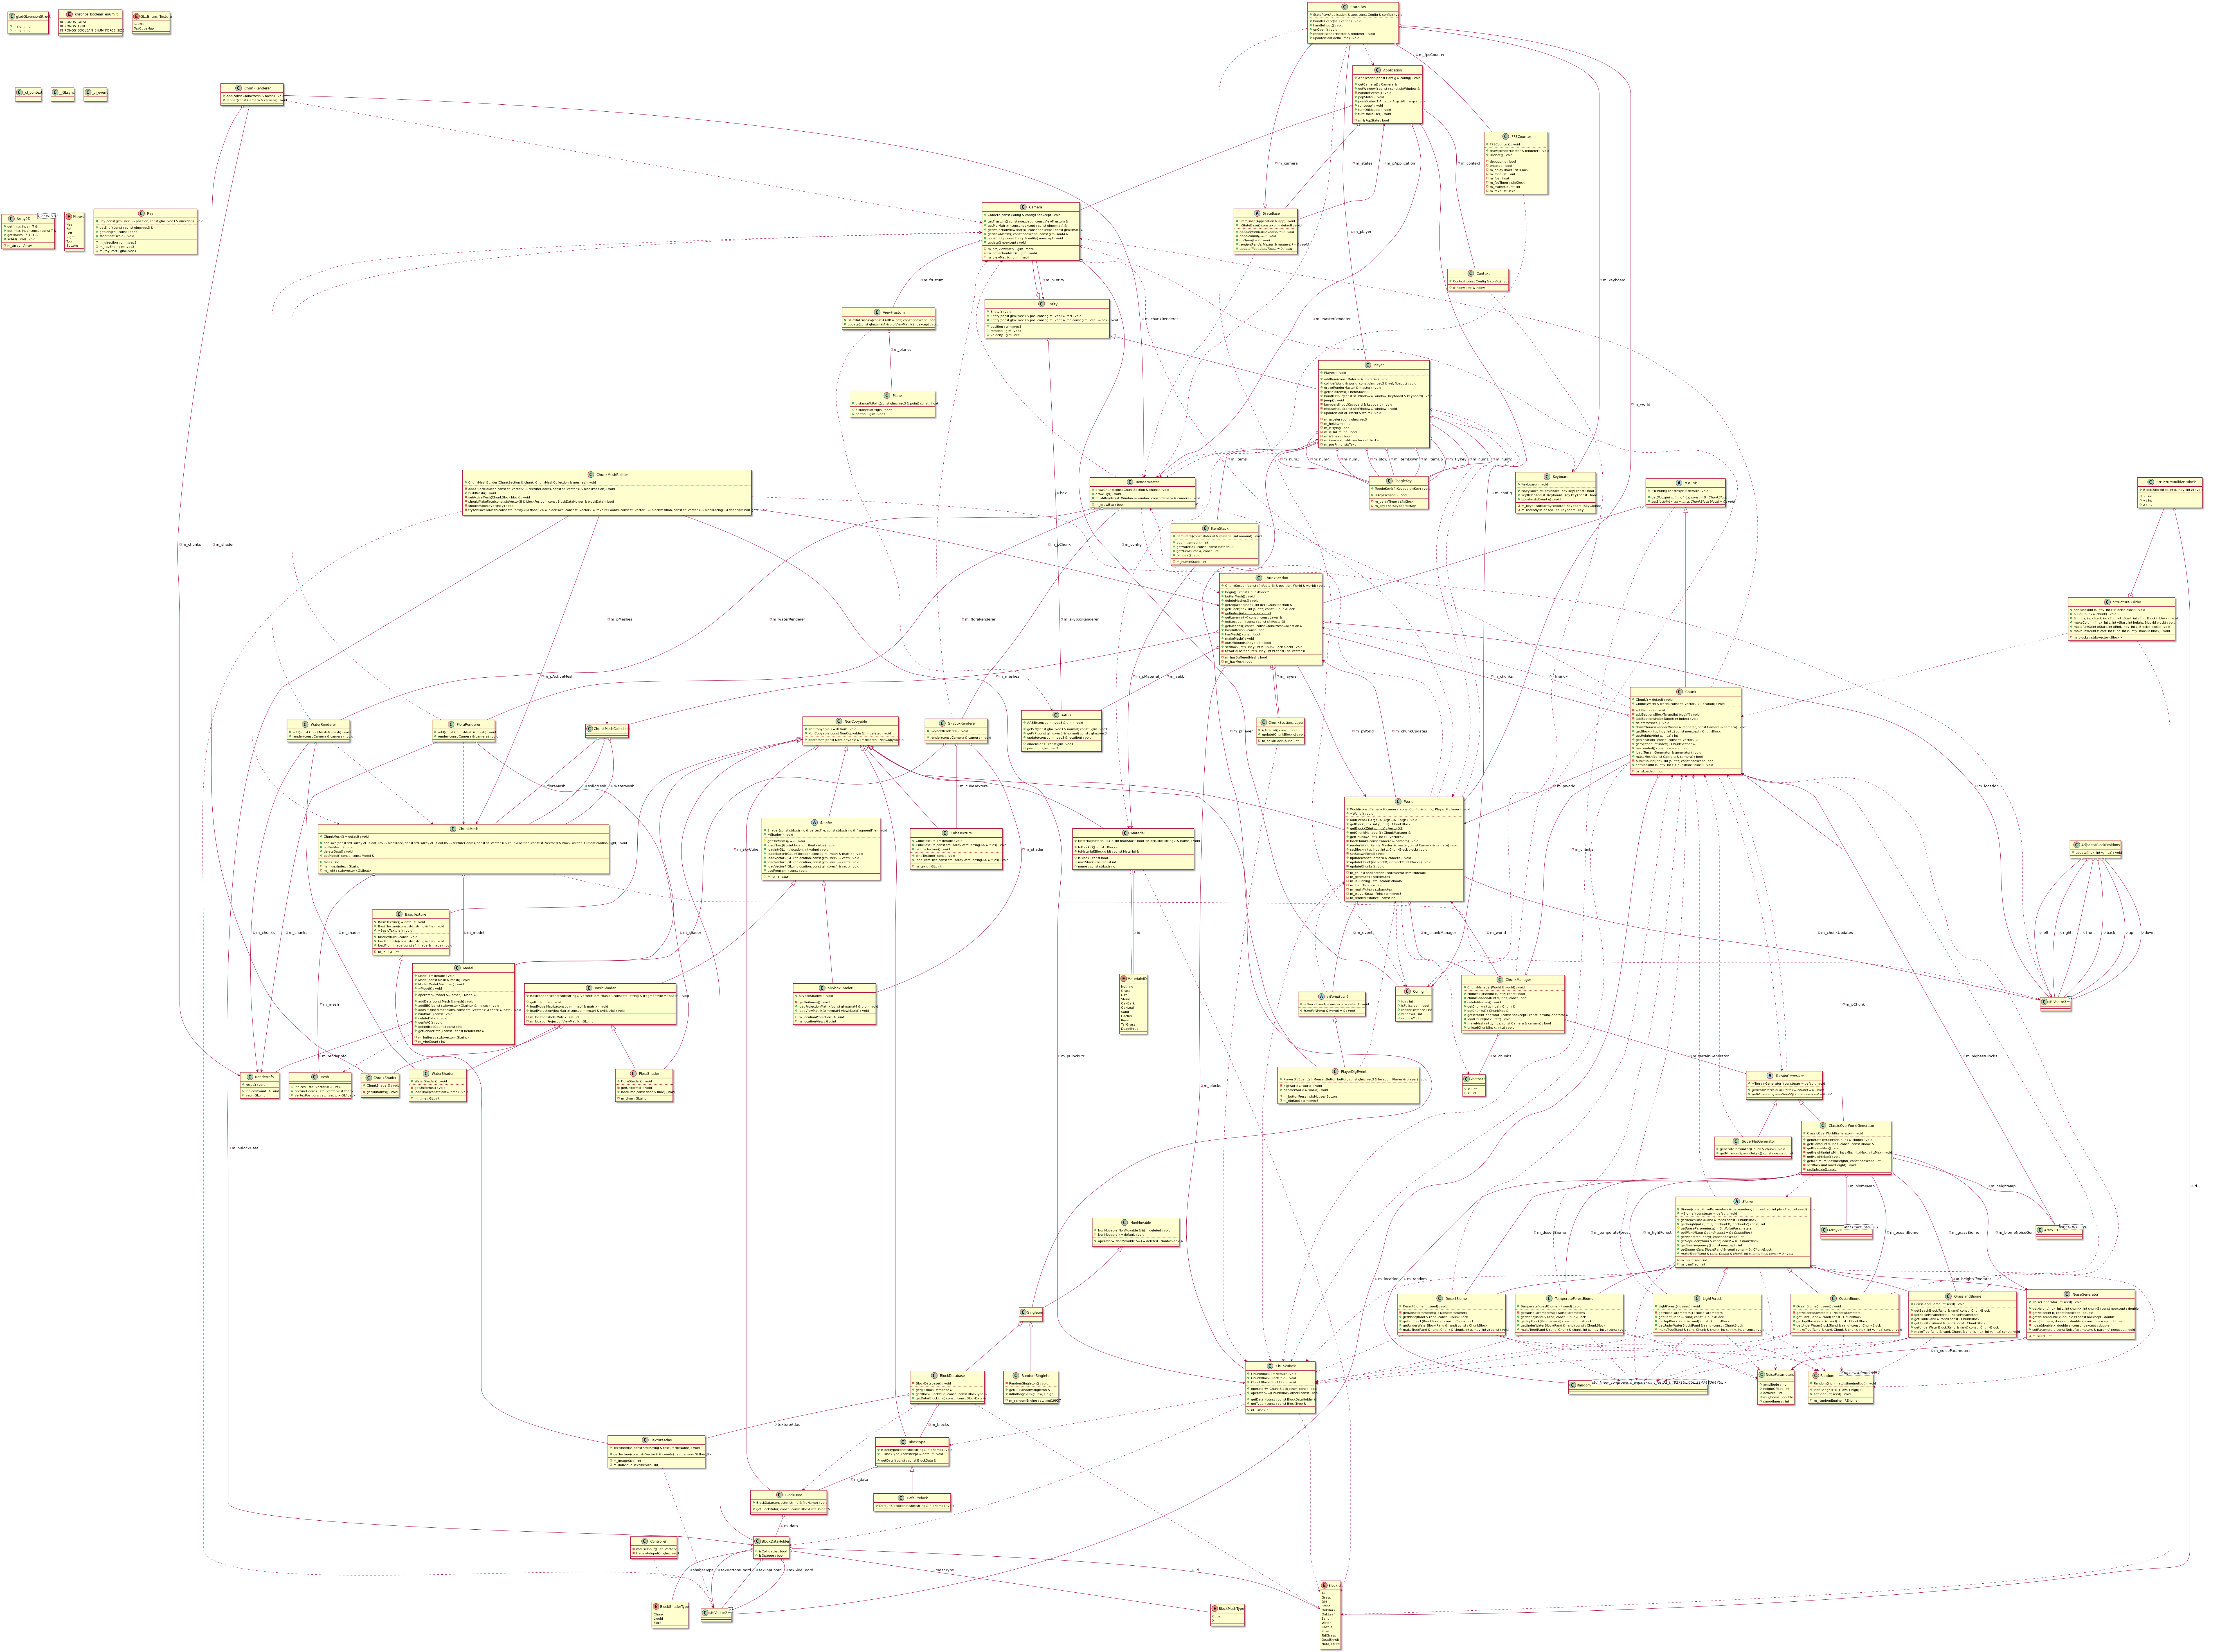
\includegraphics[width=0.95\paperwidth]{config_class.png}
  \caption{Domänenmodell}
  \label{fig:domain}
\end{figure}
\fi

%%%%%%%%%%%%%%%%%%%%%%%%%%%%%%%%%%%%%%%%%%%%%%%%%%%%%%%%%%%%%%%%%%%%%%%%%%%%%%%%

\end{document}